\begin{figure}[htb]
    \centering
    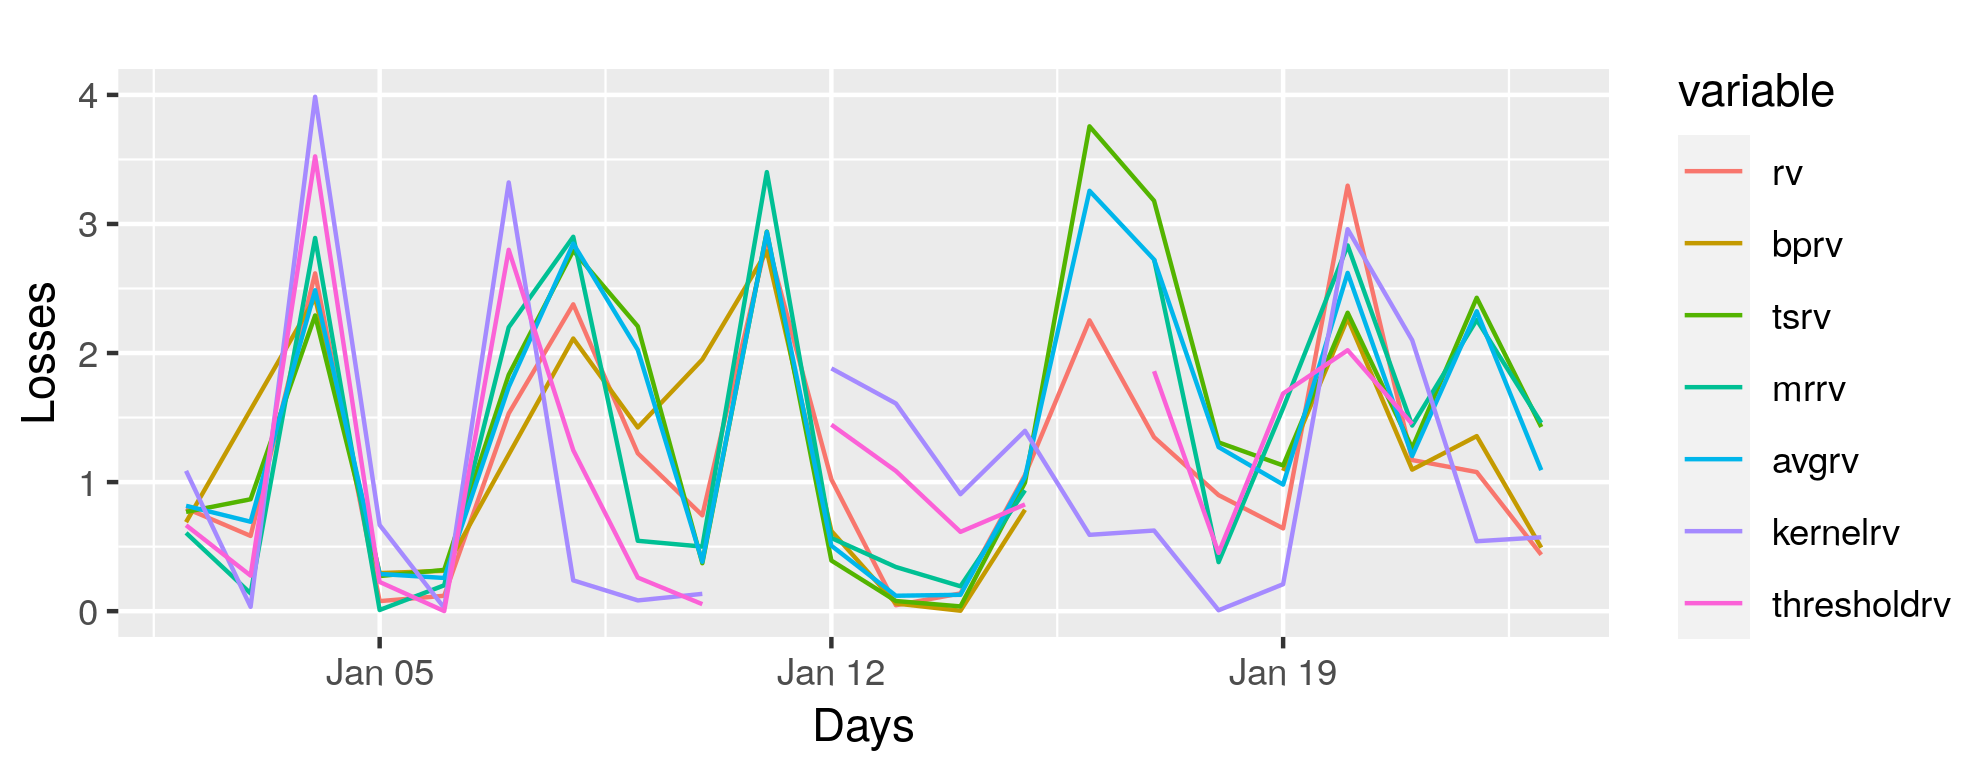
\includegraphics[width=.5\textwidth]{example-image-a}
    \caption{自带测试图片---Test image}\label{F:test-a}
    % 图片的标题应该在下方
\end{figure}

\begin{figure}[htb]
    \centering
    \begin{subfigure}[t]{.45\linewidth}
        \centering
        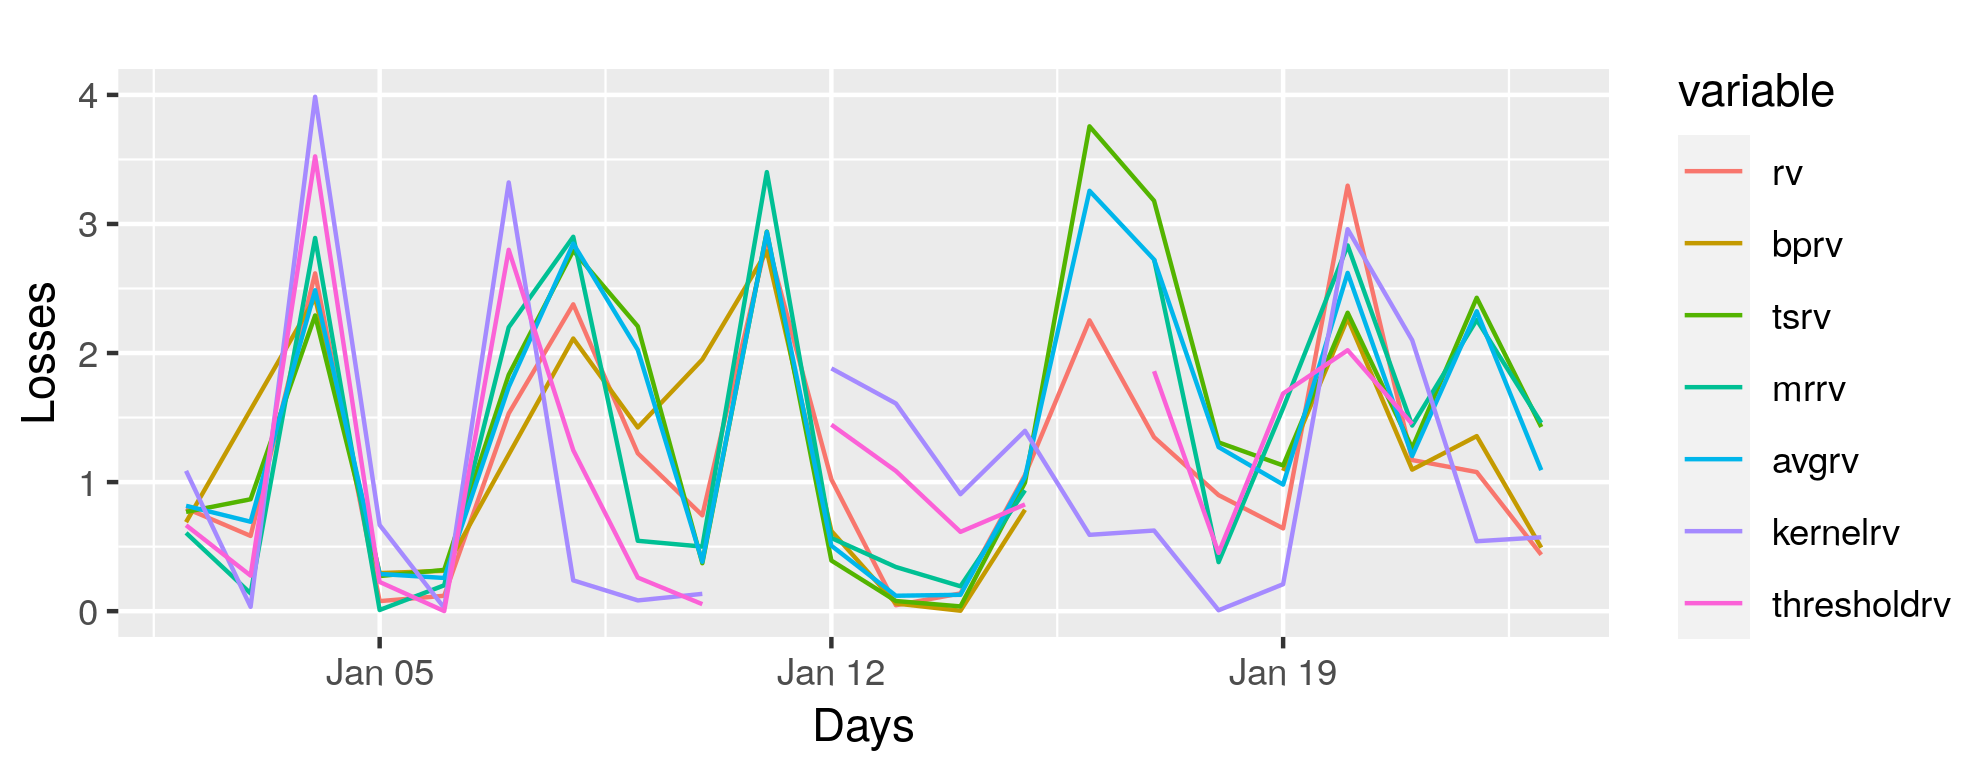
\includegraphics[width=1\textwidth]{example-image-a}
        \caption{子图-自带测试图片---Test image}\label{F:test-b-sub-a}
    \end{subfigure}
    \begin{subfigure}[t]{.45\linewidth}
        \centering
        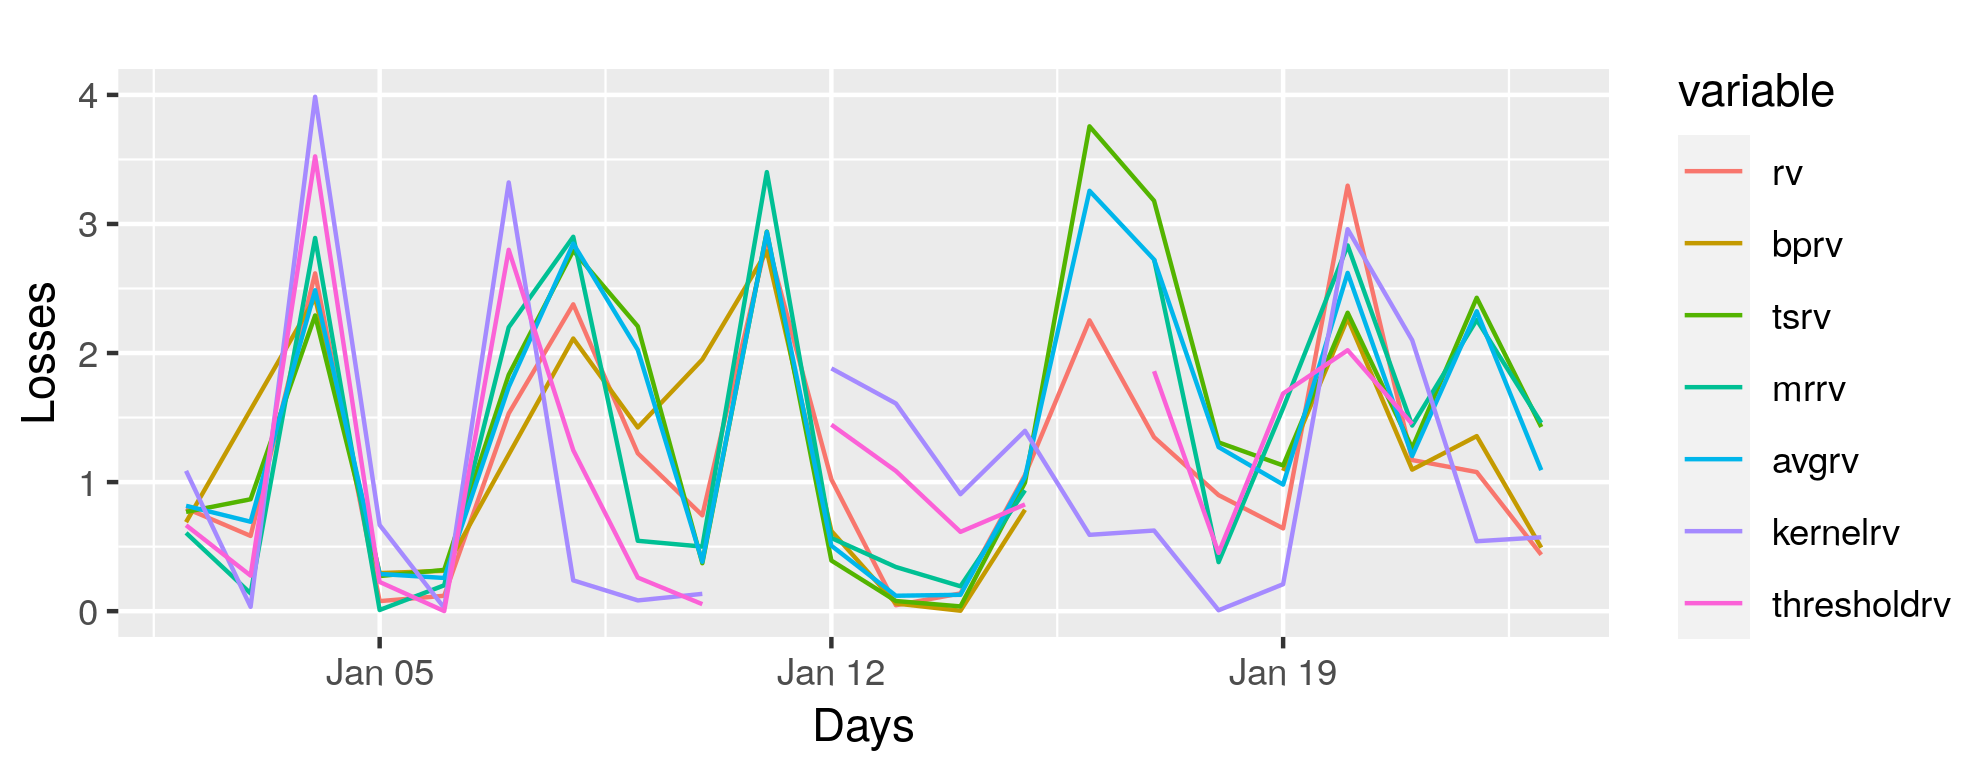
\includegraphics[width=1\textwidth]{example-image-a}
        \caption{子图-自带测试图片---Test image}\label{F:test-b-sub-b}
    \end{subfigure}
    \caption{自带测试图片---Test image}\label{F:test-b}
\end{figure}